\documentclass[twoside]{book}

% Packages required by doxygen
\usepackage{calc}
\usepackage{doxygen}
\usepackage{graphicx}
\usepackage[utf8]{inputenc}
\usepackage{makeidx}
\usepackage{multicol}
\usepackage{multirow}
\usepackage{textcomp}
\usepackage[table]{xcolor}

% Font selection
\usepackage[T1]{fontenc}
\usepackage{mathptmx}
\usepackage[scaled=.90]{helvet}
\usepackage{courier}
\usepackage{amssymb}
\usepackage{sectsty}
\renewcommand{\familydefault}{\sfdefault}
\allsectionsfont{%
  \fontseries{bc}\selectfont%
  \color{darkgray}%
}
\renewcommand{\DoxyLabelFont}{%
  \fontseries{bc}\selectfont%
  \color{darkgray}%
}

% Page & text layout
\usepackage{geometry}
\geometry{%
  a4paper,%
  top=2.5cm,%
  bottom=2.5cm,%
  left=2.5cm,%
  right=2.5cm%
}
\tolerance=750
\hfuzz=15pt
\hbadness=750
\setlength{\emergencystretch}{15pt}
\setlength{\parindent}{0cm}
\setlength{\parskip}{0.2cm}
\makeatletter
\renewcommand{\paragraph}{%
  \@startsection{paragraph}{4}{0ex}{-1.0ex}{1.0ex}{%
    \normalfont\normalsize\bfseries\SS@parafont%
  }%
}
\renewcommand{\subparagraph}{%
  \@startsection{subparagraph}{5}{0ex}{-1.0ex}{1.0ex}{%
    \normalfont\normalsize\bfseries\SS@subparafont%
  }%
}
\makeatother

% Headers & footers
\usepackage{fancyhdr}
\pagestyle{fancyplain}
\fancyhead[LE]{\fancyplain{}{\bfseries\thepage}}
\fancyhead[CE]{\fancyplain{}{}}
\fancyhead[RE]{\fancyplain{}{\bfseries\leftmark}}
\fancyhead[LO]{\fancyplain{}{\bfseries\rightmark}}
\fancyhead[CO]{\fancyplain{}{}}
\fancyhead[RO]{\fancyplain{}{\bfseries\thepage}}
\fancyfoot[LE]{\fancyplain{}{}}
\fancyfoot[CE]{\fancyplain{}{}}
\fancyfoot[RE]{\fancyplain{}{\bfseries\scriptsize Generated on Tue Mar 14 2017 22\-:44\-:54 for My Project by Doxygen }}
\fancyfoot[LO]{\fancyplain{}{\bfseries\scriptsize Generated on Tue Mar 14 2017 22\-:44\-:54 for My Project by Doxygen }}
\fancyfoot[CO]{\fancyplain{}{}}
\fancyfoot[RO]{\fancyplain{}{}}
\renewcommand{\footrulewidth}{0.4pt}
\renewcommand{\chaptermark}[1]{%
  \markboth{#1}{}%
}
\renewcommand{\sectionmark}[1]{%
  \markright{\thesection\ #1}%
}

% Indices & bibliography
\usepackage{natbib}
\usepackage[titles]{tocloft}
\setcounter{tocdepth}{3}
\setcounter{secnumdepth}{5}
\makeindex

% Hyperlinks (required, but should be loaded last)
\usepackage{ifpdf}
\ifpdf
  \usepackage[pdftex,pagebackref=true]{hyperref}
\else
  \usepackage[ps2pdf,pagebackref=true]{hyperref}
\fi
\hypersetup{%
  colorlinks=true,%
  linkcolor=blue,%
  citecolor=blue,%
  unicode%
}

% Custom commands
\newcommand{\clearemptydoublepage}{%
  \newpage{\pagestyle{empty}\cleardoublepage}%
}


%===== C O N T E N T S =====

\begin{document}

% Titlepage & ToC
\hypersetup{pageanchor=false}
\pagenumbering{roman}
\begin{titlepage}
\vspace*{7cm}
\begin{center}%
{\Large My Project }\\
\vspace*{1cm}
{\large Generated by Doxygen 1.8.6}\\
\vspace*{0.5cm}
{\small Tue Mar 14 2017 22:44:54}\\
\end{center}
\end{titlepage}
\clearemptydoublepage
\tableofcontents
\clearemptydoublepage
\pagenumbering{arabic}
\hypersetup{pageanchor=true}

%--- Begin generated contents ---
\chapter{Hierarchical Index}
\section{Class Hierarchy}
This inheritance list is sorted roughly, but not completely, alphabetically\-:\begin{DoxyCompactList}
\item \contentsline{section}{Astar}{\pageref{classAstar}}{}
\begin{DoxyCompactList}
\item \contentsline{section}{Weighted\-Astar}{\pageref{classWeightedAstar}}{}
\end{DoxyCompactList}
\item \contentsline{section}{Buildingmap}{\pageref{classBuildingmap}}{}
\item \contentsline{section}{Map}{\pageref{classMap}}{}
\item \contentsline{section}{Astar\-:\-:node}{\pageref{structAstar_1_1node}}{}
\end{DoxyCompactList}

\chapter{Class Index}
\section{Class List}
Here are the classes, structs, unions and interfaces with brief descriptions\-:\begin{DoxyCompactList}
\item\contentsline{section}{\hyperlink{classAstar}{Astar} }{\pageref{classAstar}}{}
\item\contentsline{section}{\hyperlink{classBuildingmap}{Buildingmap} }{\pageref{classBuildingmap}}{}
\item\contentsline{section}{\hyperlink{classMap}{Map} }{\pageref{classMap}}{}
\item\contentsline{section}{\hyperlink{structAstar_1_1node}{Astar\-::node} }{\pageref{structAstar_1_1node}}{}
\item\contentsline{section}{\hyperlink{classWeightedAstar}{Weighted\-Astar} }{\pageref{classWeightedAstar}}{}
\end{DoxyCompactList}

\chapter{File Index}
\section{File List}
Here is a list of all documented files with brief descriptions\-:\begin{DoxyCompactList}
\item\contentsline{section}{/home/zejiang/\-Acme-\/\-Robotics-\/\-Project/app/\hyperlink{Astar_8cpp}{Astar.\-cpp} \\*This file define several functions of $<$\-Astar$>$ class }{\pageref{Astar_8cpp}}{}
\item\contentsline{section}{/home/zejiang/\-Acme-\/\-Robotics-\/\-Project/app/\hyperlink{BuildingMap_8cpp}{Building\-Map.\-cpp} \\*This source file defines two functions of $<$\-Building\-Map$>$ class }{\pageref{BuildingMap_8cpp}}{}
\item\contentsline{section}{/home/zejiang/\-Acme-\/\-Robotics-\/\-Project/app/\hyperlink{main_8cpp}{main.\-cpp} \\*This is the main funtion for this mid-\/term peoject, it reads the user defined grid map to determine an optimal path from start to goal node }{\pageref{main_8cpp}}{}
\item\contentsline{section}{/home/zejiang/\-Acme-\/\-Robotics-\/\-Project/app/\hyperlink{Map_8cpp}{Map.\-cpp} \\*This file define two functions of $<$\-Map$>$ class }{\pageref{Map_8cpp}}{}
\item\contentsline{section}{/home/zejiang/\-Acme-\/\-Robotics-\/\-Project/app/\hyperlink{WeightedAstar_8cpp}{Weighted\-Astar.\-cpp} \\*This source file define a funtion of $<$\-Weighted\-Astar$>$ calss }{\pageref{WeightedAstar_8cpp}}{}
\item\contentsline{section}{/home/zejiang/\-Acme-\/\-Robotics-\/\-Project/include/{\bfseries Astar.\-h} }{\pageref{Astar_8h}}{}
\item\contentsline{section}{/home/zejiang/\-Acme-\/\-Robotics-\/\-Project/include/\hyperlink{BuildingMap_8h}{Building\-Map.\-h} \\*This header define the $<$\-Buildingmap$>$ calss, which is to draw the grid map }{\pageref{BuildingMap_8h}}{}
\item\contentsline{section}{/home/zejiang/\-Acme-\/\-Robotics-\/\-Project/include/\hyperlink{Map_8h}{Map.\-h} \\*This header define the $<$\-Map$>$ calss, which is to read start and goal node }{\pageref{Map_8h}}{}
\item\contentsline{section}{/home/zejiang/\-Acme-\/\-Robotics-\/\-Project/include/\hyperlink{WeightedAstar_8h}{Weighted\-Astar.\-h} \\*This header define the $<$\-Astar$>$ calss, which is an algorithm for path planning }{\pageref{WeightedAstar_8h}}{}
\end{DoxyCompactList}

\chapter{Class Documentation}
\hypertarget{classAstar}{\section{Astar Class Reference}
\label{classAstar}\index{Astar@{Astar}}
}
Inheritance diagram for Astar\-:\begin{figure}[H]
\begin{center}
\leavevmode
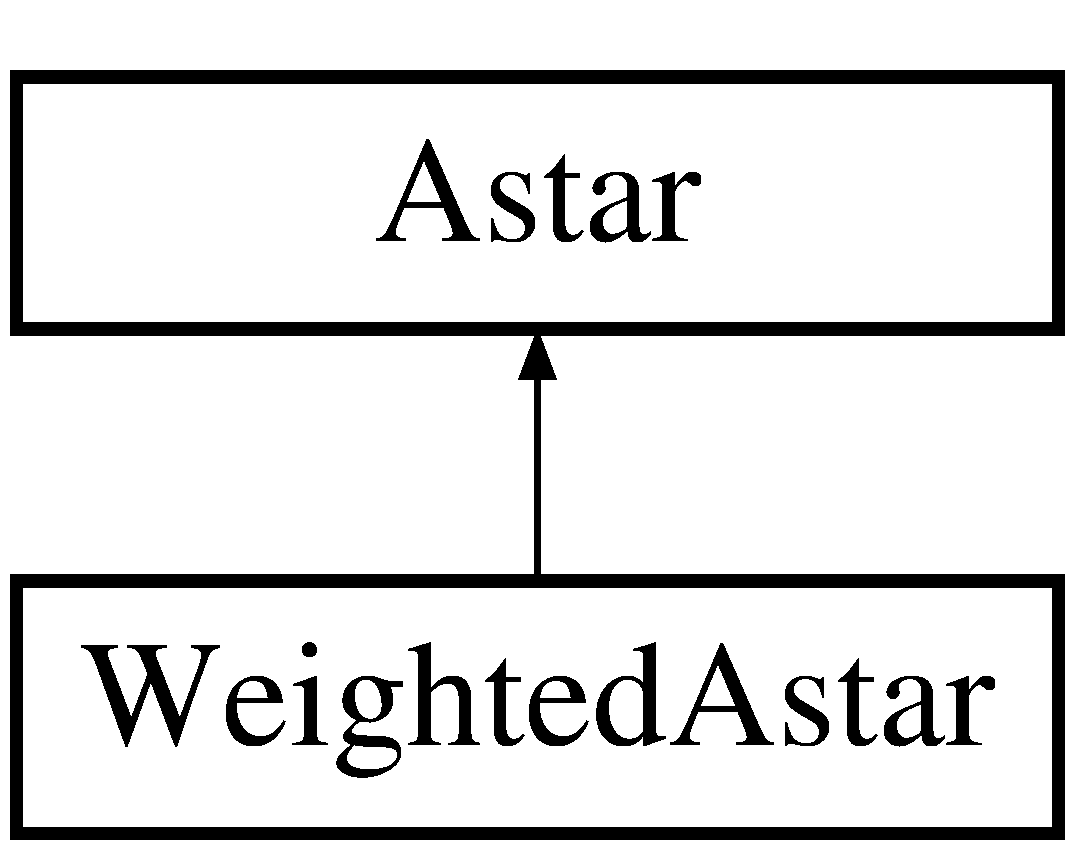
\includegraphics[height=2.000000cm]{classAstar}
\end{center}
\end{figure}
\subsection*{Classes}
\begin{DoxyCompactItemize}
\item 
struct \hyperlink{structAstar_1_1node}{node}
\end{DoxyCompactItemize}
\subsection*{Public Types}
\begin{DoxyCompactItemize}
\item 
\hypertarget{classAstar_a04e8b99eac6befb77c852c6f4155750a}{typedef std\-::pair$<$ int, int $>$ {\bfseries coordinate}}\label{classAstar_a04e8b99eac6befb77c852c6f4155750a}

\item 
\hypertarget{classAstar_a17c239ece99dd7cb5a92f5cf1404ff5d}{typedef std\-::pair$<$ double, \\*
std\-::pair$<$ int, int $>$ $>$ {\bfseries Open\-\_\-list}}\label{classAstar_a17c239ece99dd7cb5a92f5cf1404ff5d}

\end{DoxyCompactItemize}
\subsection*{Public Member Functions}
\begin{DoxyCompactItemize}
\item 
bool \hyperlink{classAstar_ae0a5f0484d586ddf52386342c7ff8b93}{is\-Valid} (const int \&x, const int \&y)
\begin{DoxyCompactList}\small\item\em Function that checks if the input coordinate is inside the grid map. \end{DoxyCompactList}\item 
bool \hyperlink{classAstar_a1613491885502d624c092c6be8cfa6d1}{is\-Unblocked} (int grid\mbox{[}$\,$\mbox{]}\mbox{[}C\-O\-L\mbox{]}, const int \&x, const int \&y)
\begin{DoxyCompactList}\small\item\em Function that checks if the grid is a block or wall something like that. \end{DoxyCompactList}\item 
bool \hyperlink{classAstar_a5525777aa1a1a6331c9c478df8c42591}{is\-Goal\-Node} (const int \&x, const int \&y, coordinate goal)
\item 
double \hyperlink{classAstar_a3f3b3457c622567a78dbf4e4aa0d62e2}{calculate\-\_\-\-H} (const int \&x, const int \&y, coordinate goal)
\begin{DoxyCompactList}\small\item\em Function that calculates the heuristic value between current node and goal node method usd here is Eucliden Distance. Other method like Diagnal Distance or Manhattan Distance are also appliable. \end{DoxyCompactList}\item 
std\-::stack$<$ coordinate $>$ \hyperlink{classAstar_a9063e14becd59719140e99554fb57822}{Generate\-Path} (\hyperlink{structAstar_1_1node}{node} nodepath\mbox{[}$\,$\mbox{]}\mbox{[}C\-O\-L\mbox{]}, coordinate goal)
\begin{DoxyCompactList}\small\item\em Function that will generate the path back from goal node to the start node and the path of the nodes will displayed on the screen. \end{DoxyCompactList}\end{DoxyCompactItemize}


\subsection{Member Function Documentation}
\hypertarget{classAstar_a3f3b3457c622567a78dbf4e4aa0d62e2}{\index{Astar@{Astar}!calculate\-\_\-\-H@{calculate\-\_\-\-H}}
\index{calculate\-\_\-\-H@{calculate\-\_\-\-H}!Astar@{Astar}}
\subsubsection[{calculate\-\_\-\-H}]{\setlength{\rightskip}{0pt plus 5cm}double Astar\-::calculate\-\_\-\-H (
\begin{DoxyParamCaption}
\item[{const int \&}]{x, }
\item[{const int \&}]{y, }
\item[{coordinate}]{goal}
\end{DoxyParamCaption}
)}}\label{classAstar_a3f3b3457c622567a78dbf4e4aa0d62e2}


Function that calculates the heuristic value between current node and goal node method usd here is Eucliden Distance. Other method like Diagnal Distance or Manhattan Distance are also appliable. 


\begin{DoxyParams}{Parameters}
{\em two} & int x and y, coordinate of gaol \\
\hline
\end{DoxyParams}
\begin{DoxyReturn}{Returns}
doule 
\end{DoxyReturn}
\hypertarget{classAstar_a9063e14becd59719140e99554fb57822}{\index{Astar@{Astar}!Generate\-Path@{Generate\-Path}}
\index{Generate\-Path@{Generate\-Path}!Astar@{Astar}}
\subsubsection[{Generate\-Path}]{\setlength{\rightskip}{0pt plus 5cm}std\-::stack$<$ coordinate $>$ Astar\-::\-Generate\-Path (
\begin{DoxyParamCaption}
\item[{{\bf node}}]{nodepath\mbox{[}$\,$\mbox{]}\mbox{[}\-C\-O\-L\mbox{]}, }
\item[{coordinate}]{goal}
\end{DoxyParamCaption}
)}}\label{classAstar_a9063e14becd59719140e99554fb57822}


Function that will generate the path back from goal node to the start node and the path of the nodes will displayed on the screen. 


\begin{DoxyParams}{Parameters}
{\em nodepath} & and goal coordinate \\
\hline
\end{DoxyParams}
\begin{DoxyReturn}{Returns}
stack$<$coordinate$>$ 
\end{DoxyReturn}
\hypertarget{classAstar_a5525777aa1a1a6331c9c478df8c42591}{\index{Astar@{Astar}!is\-Goal\-Node@{is\-Goal\-Node}}
\index{is\-Goal\-Node@{is\-Goal\-Node}!Astar@{Astar}}
\subsubsection[{is\-Goal\-Node}]{\setlength{\rightskip}{0pt plus 5cm}bool Astar\-::is\-Goal\-Node (
\begin{DoxyParamCaption}
\item[{const int \&}]{x, }
\item[{const int \&}]{y, }
\item[{coordinate}]{goal}
\end{DoxyParamCaption}
)}}\label{classAstar_a5525777aa1a1a6331c9c478df8c42591}
@ Funtion that checks if it is the goal node 
\begin{DoxyParams}{Parameters}
{\em two} & int x and y, goal coordinate \\
\hline
\end{DoxyParams}
\begin{DoxyReturn}{Returns}
boolean,ture or false 
\end{DoxyReturn}
\hypertarget{classAstar_a1613491885502d624c092c6be8cfa6d1}{\index{Astar@{Astar}!is\-Unblocked@{is\-Unblocked}}
\index{is\-Unblocked@{is\-Unblocked}!Astar@{Astar}}
\subsubsection[{is\-Unblocked}]{\setlength{\rightskip}{0pt plus 5cm}bool Astar\-::is\-Unblocked (
\begin{DoxyParamCaption}
\item[{int}]{grid\mbox{[}$\,$\mbox{]}\mbox{[}\-C\-O\-L\mbox{]}, }
\item[{const int \&}]{x, }
\item[{const int \&}]{y}
\end{DoxyParamCaption}
)}}\label{classAstar_a1613491885502d624c092c6be8cfa6d1}


Function that checks if the grid is a block or wall something like that. 


\begin{DoxyParams}{Parameters}
{\em grid\mbox{[}10\mbox{]}\mbox{[}10\mbox{]},coordinate} & x and y, int \\
\hline
\end{DoxyParams}
\begin{DoxyReturn}{Returns}
boolean ture or false 
\end{DoxyReturn}
\hypertarget{classAstar_ae0a5f0484d586ddf52386342c7ff8b93}{\index{Astar@{Astar}!is\-Valid@{is\-Valid}}
\index{is\-Valid@{is\-Valid}!Astar@{Astar}}
\subsubsection[{is\-Valid}]{\setlength{\rightskip}{0pt plus 5cm}bool Astar\-::is\-Valid (
\begin{DoxyParamCaption}
\item[{const int \&}]{x, }
\item[{const int \&}]{y}
\end{DoxyParamCaption}
)}}\label{classAstar_ae0a5f0484d586ddf52386342c7ff8b93}


Function that checks if the input coordinate is inside the grid map. 


\begin{DoxyParams}{Parameters}
{\em two} & integars \\
\hline
\end{DoxyParams}
\begin{DoxyReturn}{Returns}
ture or false 
\end{DoxyReturn}


The documentation for this class was generated from the following files\-:\begin{DoxyCompactItemize}
\item 
/home/zejiang/\-Acme-\/\-Robotics-\/\-Project/include/Astar.\-h\item 
/home/zejiang/\-Acme-\/\-Robotics-\/\-Project/app/\hyperlink{Astar_8cpp}{Astar.\-cpp}\end{DoxyCompactItemize}

\hypertarget{classBuildingmap}{\section{Buildingmap Class Reference}
\label{classBuildingmap}\index{Buildingmap@{Buildingmap}}
}
\subsection*{Public Member Functions}
\begin{DoxyCompactItemize}
\item 
cv\-::\-Mat \hyperlink{classBuildingmap_a6fdcdfd5c371e0c43f39ff6e4ae99bc1}{draw\-Grids} (int grid\mbox{[}R\-O\-W\mbox{]}\mbox{[}C\-O\-L\mbox{]}, Astar\-::coordinate start, Astar\-::coordinate goal)
\begin{DoxyCompactList}\small\item\em Funtion that draw the grid map by using Opencv, walls will be black start and goal node are R\-G\-B\mbox{[}0,255,255\mbox{]}. \end{DoxyCompactList}\item 
cv\-::\-Mat \hyperlink{classBuildingmap_a9d149d9b85adfe94a91bed65736c0ed9}{draw\-Path} (std\-::stack$<$ Astar\-::coordinate $>$ Path, cv\-::\-Mat Background)
\begin{DoxyCompactList}\small\item\em Funtion that draw the path node which are R\-G\-B\mbox{[}0,255,255\mbox{]}. \end{DoxyCompactList}\end{DoxyCompactItemize}


\subsection{Member Function Documentation}
\hypertarget{classBuildingmap_a6fdcdfd5c371e0c43f39ff6e4ae99bc1}{\index{Buildingmap@{Buildingmap}!draw\-Grids@{draw\-Grids}}
\index{draw\-Grids@{draw\-Grids}!Buildingmap@{Buildingmap}}
\subsubsection[{draw\-Grids}]{\setlength{\rightskip}{0pt plus 5cm}cv\-::\-Mat Buildingmap\-::draw\-Grids (
\begin{DoxyParamCaption}
\item[{int}]{grid\mbox{[}\-R\-O\-W\mbox{]}\mbox{[}\-C\-O\-L\mbox{]}, }
\item[{Astar\-::coordinate}]{start, }
\item[{Astar\-::coordinate}]{goal}
\end{DoxyParamCaption}
)}}\label{classBuildingmap_a6fdcdfd5c371e0c43f39ff6e4ae99bc1}


Funtion that draw the grid map by using Opencv, walls will be black start and goal node are R\-G\-B\mbox{[}0,255,255\mbox{]}. 


\begin{DoxyParams}{Parameters}
{\em int} & grid\mbox{[}\mbox{]}\mbox{[}\mbox{]}, start and goal coordinate \\
\hline
\end{DoxyParams}
\begin{DoxyReturn}{Returns}
cv\-::\-Mat, an image show map including walls, start, goal node 
\end{DoxyReturn}
\hypertarget{classBuildingmap_a9d149d9b85adfe94a91bed65736c0ed9}{\index{Buildingmap@{Buildingmap}!draw\-Path@{draw\-Path}}
\index{draw\-Path@{draw\-Path}!Buildingmap@{Buildingmap}}
\subsubsection[{draw\-Path}]{\setlength{\rightskip}{0pt plus 5cm}cv\-::\-Mat Buildingmap\-::draw\-Path (
\begin{DoxyParamCaption}
\item[{std\-::stack$<$ Astar\-::coordinate $>$}]{Path, }
\item[{cv\-::\-Mat}]{Background}
\end{DoxyParamCaption}
)}}\label{classBuildingmap_a9d149d9b85adfe94a91bed65736c0ed9}


Funtion that draw the path node which are R\-G\-B\mbox{[}0,255,255\mbox{]}. 


\begin{DoxyParams}{Parameters}
{\em Path} & nodes in stack $<$coordinate$>$, map image Background, in cv\-::\-Mat \\
\hline
\end{DoxyParams}
\begin{DoxyReturn}{Returns}
cv\-::\-Mat, an image show map including walls, start, goal node anb path 
\end{DoxyReturn}


The documentation for this class was generated from the following files\-:\begin{DoxyCompactItemize}
\item 
/home/zejiang/\-Acme-\/\-Robotics-\/\-Project/include/\hyperlink{BuildingMap_8h}{Building\-Map.\-h}\item 
/home/zejiang/\-Acme-\/\-Robotics-\/\-Project/app/\hyperlink{BuildingMap_8cpp}{Building\-Map.\-cpp}\end{DoxyCompactItemize}

\hypertarget{classMap}{\section{Map Class Reference}
\label{classMap}\index{Map@{Map}}
}
\subsection*{Public Member Functions}
\begin{DoxyCompactItemize}
\item 
Astar\-::coordinate \hyperlink{classMap_a7a5eb2bb2a4f6e7002aefea0f1516a2e}{Set\-Start} (const int \&x, const int \&y)
\begin{DoxyCompactList}\small\item\em This function read two integar and make them as the 2\-D coordinate of the node. \end{DoxyCompactList}\item 
Astar\-::coordinate \hyperlink{classMap_a360fe819c070cdc5a4346dcbe84d07b4}{Set\-Goal} (const int \&x, const int \&y)
\begin{DoxyCompactList}\small\item\em Same as last funtion, it returns the coordinate of goal node. \end{DoxyCompactList}\end{DoxyCompactItemize}


\subsection{Member Function Documentation}
\hypertarget{classMap_a360fe819c070cdc5a4346dcbe84d07b4}{\index{Map@{Map}!Set\-Goal@{Set\-Goal}}
\index{Set\-Goal@{Set\-Goal}!Map@{Map}}
\subsubsection[{Set\-Goal}]{\setlength{\rightskip}{0pt plus 5cm}Astar\-::coordinate Map\-::\-Set\-Goal (
\begin{DoxyParamCaption}
\item[{const int \&}]{x, }
\item[{const int \&}]{y}
\end{DoxyParamCaption}
)}}\label{classMap_a360fe819c070cdc5a4346dcbe84d07b4}


Same as last funtion, it returns the coordinate of goal node. 


\begin{DoxyParams}{Parameters}
{\em two} & integars x and y \\
\hline
\end{DoxyParams}
\begin{DoxyReturn}{Returns}
coordinate pair$<$x,y$>$ 
\end{DoxyReturn}
\hypertarget{classMap_a7a5eb2bb2a4f6e7002aefea0f1516a2e}{\index{Map@{Map}!Set\-Start@{Set\-Start}}
\index{Set\-Start@{Set\-Start}!Map@{Map}}
\subsubsection[{Set\-Start}]{\setlength{\rightskip}{0pt plus 5cm}Astar\-::coordinate Map\-::\-Set\-Start (
\begin{DoxyParamCaption}
\item[{const int \&}]{x, }
\item[{const int \&}]{y}
\end{DoxyParamCaption}
)}}\label{classMap_a7a5eb2bb2a4f6e7002aefea0f1516a2e}


This function read two integar and make them as the 2\-D coordinate of the node. 


\begin{DoxyParams}{Parameters}
{\em x} & and y, both are int, which represent the location of the start node \\
\hline
\end{DoxyParams}
\begin{DoxyReturn}{Returns}
coordinate pair$<$x,y$>$ 
\end{DoxyReturn}


The documentation for this class was generated from the following files\-:\begin{DoxyCompactItemize}
\item 
/home/zejiang/\-Acme-\/\-Robotics-\/\-Project/include/\hyperlink{Map_8h}{Map.\-h}\item 
/home/zejiang/\-Acme-\/\-Robotics-\/\-Project/app/\hyperlink{Map_8cpp}{Map.\-cpp}\end{DoxyCompactItemize}

\hypertarget{structAstar_1_1node}{\section{Astar\-:\-:node Struct Reference}
\label{structAstar_1_1node}\index{Astar\-::node@{Astar\-::node}}
}
\subsection*{Public Attributes}
\begin{DoxyCompactItemize}
\item 
\hypertarget{structAstar_1_1node_a171ad5aa886b859fc0103dae466e38eb}{int {\bfseries parent\-\_\-x}}\label{structAstar_1_1node_a171ad5aa886b859fc0103dae466e38eb}

\item 
\hypertarget{structAstar_1_1node_a89a62ffd7014525b6cbbf6fe98f88d47}{int {\bfseries parent\-\_\-y}}\label{structAstar_1_1node_a89a62ffd7014525b6cbbf6fe98f88d47}

\item 
\hypertarget{structAstar_1_1node_af030469fe3c3cef6df69a9f2e2632c21}{double {\bfseries F}}\label{structAstar_1_1node_af030469fe3c3cef6df69a9f2e2632c21}

\item 
\hypertarget{structAstar_1_1node_a6bf6c47fdc529c05bd496b1e1640679e}{double {\bfseries H}}\label{structAstar_1_1node_a6bf6c47fdc529c05bd496b1e1640679e}

\item 
\hypertarget{structAstar_1_1node_a74eb145e28f56e540e511b9431543d97}{double {\bfseries G}}\label{structAstar_1_1node_a74eb145e28f56e540e511b9431543d97}

\end{DoxyCompactItemize}


The documentation for this struct was generated from the following file\-:\begin{DoxyCompactItemize}
\item 
/home/zejiang/\-Acme-\/\-Robotics-\/\-Project/include/Astar.\-h\end{DoxyCompactItemize}

\hypertarget{classWeightedAstar}{\section{Weighted\-Astar Class Reference}
\label{classWeightedAstar}\index{Weighted\-Astar@{Weighted\-Astar}}
}
Inheritance diagram for Weighted\-Astar\-:\begin{figure}[H]
\begin{center}
\leavevmode
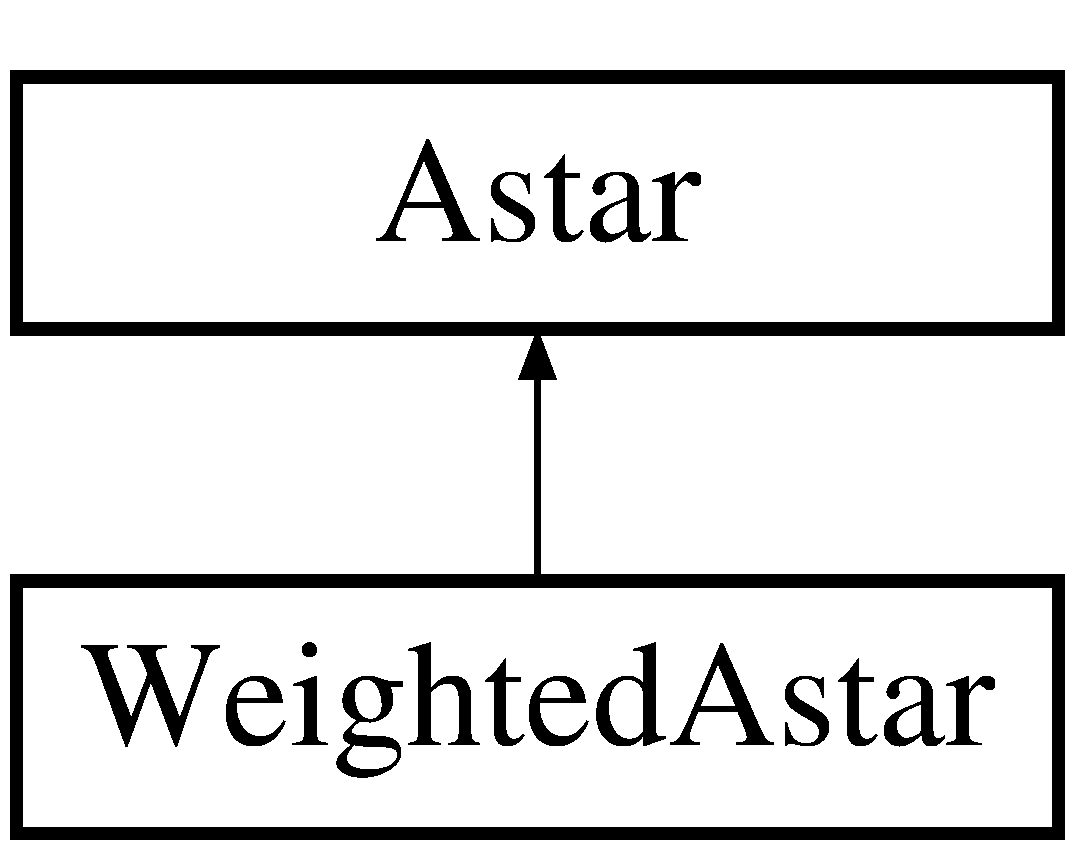
\includegraphics[height=2.000000cm]{classWeightedAstar}
\end{center}
\end{figure}
\subsection*{Public Member Functions}
\begin{DoxyCompactItemize}
\item 
std\-::stack$<$ coordinate $>$ \hyperlink{classWeightedAstar_a1794edfb3807236774434e7bc152bce2}{Weighted\-A} (int grid\mbox{[}$\,$\mbox{]}\mbox{[}C\-O\-L\mbox{]}, coordinate start, coordinate goal, const int \&weight)
\end{DoxyCompactItemize}
\subsection*{Additional Inherited Members}


\subsection{Member Function Documentation}
\hypertarget{classWeightedAstar_a1794edfb3807236774434e7bc152bce2}{\index{Weighted\-Astar@{Weighted\-Astar}!Weighted\-A@{Weighted\-A}}
\index{Weighted\-A@{Weighted\-A}!WeightedAstar@{Weighted\-Astar}}
\subsubsection[{Weighted\-A}]{\setlength{\rightskip}{0pt plus 5cm}std\-::stack$<$ Astar\-::coordinate $>$ Weighted\-Astar\-::\-Weighted\-A (
\begin{DoxyParamCaption}
\item[{int}]{grid\mbox{[}$\,$\mbox{]}\mbox{[}\-C\-O\-L\mbox{]}, }
\item[{coordinate}]{start, }
\item[{coordinate}]{goal, }
\item[{const int \&}]{weight}
\end{DoxyParamCaption}
)}}\label{classWeightedAstar_a1794edfb3807236774434e7bc152bce2}
brief Funtion that generate a path from start to goal ndoe by using a path planing algorithm called \hyperlink{classWeightedAstar}{Weighted\-Astar} 
\begin{DoxyParams}{Parameters}
{\em int} & grid\mbox{[}10\mbox{]}\mbox{[}10\mbox{]}, a 10 by 10 grid map, locaion of start and goal node, weight , an integar \\
\hline
\end{DoxyParams}
\begin{DoxyReturn}{Returns}
stack $<$coordinate$>$ lolation of the path node 
\end{DoxyReturn}


The documentation for this class was generated from the following files\-:\begin{DoxyCompactItemize}
\item 
/home/zejiang/\-Acme-\/\-Robotics-\/\-Project/include/\hyperlink{WeightedAstar_8h}{Weighted\-Astar.\-h}\item 
/home/zejiang/\-Acme-\/\-Robotics-\/\-Project/app/\hyperlink{WeightedAstar_8cpp}{Weighted\-Astar.\-cpp}\end{DoxyCompactItemize}

\chapter{File Documentation}
\hypertarget{Astar_8cpp}{\section{/home/zejiang/\-Acme-\/\-Robotics-\/\-Project/app/\-Astar.cpp File Reference}
\label{Astar_8cpp}\index{/home/zejiang/\-Acme-\/\-Robotics-\/\-Project/app/\-Astar.\-cpp@{/home/zejiang/\-Acme-\/\-Robotics-\/\-Project/app/\-Astar.\-cpp}}
}


This file define several functions of $<$\-Astar$>$ class.  


{\ttfamily \#include $<$iostream$>$}\\*
{\ttfamily \#include $<$set$>$}\\*
{\ttfamily \#include $<$vector$>$}\\*
{\ttfamily \#include $<$stack$>$}\\*
{\ttfamily \#include \char`\"{}Astar.\-h\char`\"{}}\\*
{\ttfamily \#include $<$cmath$>$}\\*
{\ttfamily \#include $<$utility$>$}\\*
\subsection*{Typedefs}
\begin{DoxyCompactItemize}
\item 
\hypertarget{Astar_8cpp_a23f8a35d095145835a835a5a6c3df6d6}{typedef std\-::pair$<$ int, int $>$ {\bfseries coordinate}}\label{Astar_8cpp_a23f8a35d095145835a835a5a6c3df6d6}

\end{DoxyCompactItemize}


\subsection{Detailed Description}
This file define several functions of $<$\-Astar$>$ class. (C) 2017 Zejiang Zeng -\/ All Rights Reserved You may use, distribute and modify this code under the terms of the M\-I\-T license, please visit \-: \href{https://github.com/zzjkf2009/Acme-Robotics-Project/blob/master/LICENSE}{\tt https\-://github.\-com/zzjkf2009/\-Acme-\/\-Robotics-\/\-Project/blob/master/\-L\-I\-C\-E\-N\-S\-E} 
\hypertarget{BuildingMap_8cpp}{\section{/home/zejiang/\-Acme-\/\-Robotics-\/\-Project/app/\-Building\-Map.cpp File Reference}
\label{BuildingMap_8cpp}\index{/home/zejiang/\-Acme-\/\-Robotics-\/\-Project/app/\-Building\-Map.\-cpp@{/home/zejiang/\-Acme-\/\-Robotics-\/\-Project/app/\-Building\-Map.\-cpp}}
}


This source file defines two functions of $<$\-Building\-Map$>$ class.  


{\ttfamily \#include $<$opencv2/opencv.\-hpp$>$}\\*
{\ttfamily \#include $<$cmath$>$}\\*
{\ttfamily \#include $<$stack$>$}\\*
{\ttfamily \#include \char`\"{}Building\-Map.\-h\char`\"{}}\\*
{\ttfamily \#include $<$utility$>$}\\*
\subsection*{Typedefs}
\begin{DoxyCompactItemize}
\item 
\hypertarget{BuildingMap_8cpp_a23f8a35d095145835a835a5a6c3df6d6}{typedef std\-::pair$<$ int, int $>$ {\bfseries coordinate}}\label{BuildingMap_8cpp_a23f8a35d095145835a835a5a6c3df6d6}

\end{DoxyCompactItemize}


\subsection{Detailed Description}
This source file defines two functions of $<$\-Building\-Map$>$ class. (C) 2017 Zejiang Zeng -\/ All Rights Reserved You may use, distribute and modify this code under the terms of the M\-I\-T license, please visit \-: \href{https://github.com/zzjkf2009/Acme-Robotics-Project/blob/master/LICENSE}{\tt https\-://github.\-com/zzjkf2009/\-Acme-\/\-Robotics-\/\-Project/blob/master/\-L\-I\-C\-E\-N\-S\-E} 
\hypertarget{main_8cpp}{\section{/home/zejiang/\-Acme-\/\-Robotics-\/\-Project/app/main.cpp File Reference}
\label{main_8cpp}\index{/home/zejiang/\-Acme-\/\-Robotics-\/\-Project/app/main.\-cpp@{/home/zejiang/\-Acme-\/\-Robotics-\/\-Project/app/main.\-cpp}}
}


This is the main funtion for this mid-\/term peoject, it reads the user defined grid map to determine an optimal path from start to goal node.  


{\ttfamily \#include $<$opencv2/opencv.\-hpp$>$}\\*
{\ttfamily \#include $<$iostream$>$}\\*
{\ttfamily \#include $<$set$>$}\\*
{\ttfamily \#include $<$vector$>$}\\*
{\ttfamily \#include $<$stack$>$}\\*
{\ttfamily \#include \char`\"{}Building\-Map.\-h\char`\"{}}\\*
{\ttfamily \#include \char`\"{}Weighted\-Astar.\-h\char`\"{}}\\*
{\ttfamily \#include \char`\"{}Map.\-h\char`\"{}}\\*
{\ttfamily \#include \char`\"{}Astar.\-h\char`\"{}}\\*
\subsection*{Functions}
\begin{DoxyCompactItemize}
\item 
\hypertarget{main_8cpp_ae66f6b31b5ad750f1fe042a706a4e3d4}{int {\bfseries main} ()}\label{main_8cpp_ae66f6b31b5ad750f1fe042a706a4e3d4}

\end{DoxyCompactItemize}


\subsection{Detailed Description}
This is the main funtion for this mid-\/term peoject, it reads the user defined grid map to determine an optimal path from start to goal node. (C) 2017 Zejiang Zeng -\/ All Rights Reserved You may use, distribute and modify this code under the terms of the M\-I\-T license, please visit \-: \href{https://github.com/zzjkf2009/Acme-Robotics-Project/blob/master/LICENSE}{\tt https\-://github.\-com/zzjkf2009/\-Acme-\/\-Robotics-\/\-Project/blob/master/\-L\-I\-C\-E\-N\-S\-E} \begin{DoxyReturn}{Returns}
the path from start to goal node will be displayed on the screen and map with path will be showed in a image 
\end{DoxyReturn}

\hypertarget{Map_8cpp}{\section{/home/zejiang/\-Acme-\/\-Robotics-\/\-Project/app/\-Map.cpp File Reference}
\label{Map_8cpp}\index{/home/zejiang/\-Acme-\/\-Robotics-\/\-Project/app/\-Map.\-cpp@{/home/zejiang/\-Acme-\/\-Robotics-\/\-Project/app/\-Map.\-cpp}}
}


This file define two functions of $<$\-Map$>$ class.  


{\ttfamily \#include \char`\"{}Map.\-h\char`\"{}}\\*
{\ttfamily \#include \char`\"{}Astar.\-h\char`\"{}}\\*
{\ttfamily \#include $<$utility$>$}\\*


\subsection{Detailed Description}
This file define two functions of $<$\-Map$>$ class. (C) 2017 Zejiang Zeng -\/ All Rights Reserved You may use, distribute and modify this code under the terms of the M\-I\-T license, please visit \-: \href{https://github.com/zzjkf2009/Acme-Robotics-Project/blob/master/LICENSE}{\tt https\-://github.\-com/zzjkf2009/\-Acme-\/\-Robotics-\/\-Project/blob/master/\-L\-I\-C\-E\-N\-S\-E} 
\hypertarget{WeightedAstar_8cpp}{\section{/home/zejiang/\-Acme-\/\-Robotics-\/\-Project/app/\-Weighted\-Astar.cpp File Reference}
\label{WeightedAstar_8cpp}\index{/home/zejiang/\-Acme-\/\-Robotics-\/\-Project/app/\-Weighted\-Astar.\-cpp@{/home/zejiang/\-Acme-\/\-Robotics-\/\-Project/app/\-Weighted\-Astar.\-cpp}}
}


This source file define a funtion of $<$\-Weighted\-Astar$>$ calss.  


{\ttfamily \#include $<$iostream$>$}\\*
{\ttfamily \#include $<$set$>$}\\*
{\ttfamily \#include $<$vector$>$}\\*
{\ttfamily \#include $<$stack$>$}\\*
{\ttfamily \#include \char`\"{}Weighted\-Astar.\-h\char`\"{}}\\*
{\ttfamily \#include \char`\"{}Astar.\-h\char`\"{}}\\*
{\ttfamily \#include $<$cmath$>$}\\*
{\ttfamily \#include $<$cstring$>$}\\*
{\ttfamily \#include $<$utility$>$}\\*


\subsection{Detailed Description}
This source file define a funtion of $<$\-Weighted\-Astar$>$ calss. (C) 2017 Zejiang Zeng -\/ All Rights Reserved You may use, distribute and modify this code under the terms of the M\-I\-T license, please visit \-: \href{https://github.com/zzjkf2009/Acme-Robotics-Project/blob/master/LICENSE}{\tt https\-://github.\-com/zzjkf2009/\-Acme-\/\-Robotics-\/\-Project/blob/master/\-L\-I\-C\-E\-N\-S\-E} 
\hypertarget{BuildingMap_8h}{\section{/home/zejiang/\-Acme-\/\-Robotics-\/\-Project/include/\-Building\-Map.h File Reference}
\label{BuildingMap_8h}\index{/home/zejiang/\-Acme-\/\-Robotics-\/\-Project/include/\-Building\-Map.\-h@{/home/zejiang/\-Acme-\/\-Robotics-\/\-Project/include/\-Building\-Map.\-h}}
}


This header define the $<$\-Buildingmap$>$ calss, which is to draw the grid map.  


{\ttfamily \#include $<$opencv2/opencv.\-hpp$>$}\\*
{\ttfamily \#include $<$cmath$>$}\\*
{\ttfamily \#include $<$stack$>$}\\*
{\ttfamily \#include \char`\"{}Astar.\-h\char`\"{}}\\*
\subsection*{Classes}
\begin{DoxyCompactItemize}
\item 
class \hyperlink{classBuildingmap}{Buildingmap}
\end{DoxyCompactItemize}
\subsection*{Macros}
\begin{DoxyCompactItemize}
\item 
\hypertarget{BuildingMap_8h_ac6f18a9e1d00b4637522b1b469a92021}{\#define {\bfseries R\-O\-W}~10}\label{BuildingMap_8h_ac6f18a9e1d00b4637522b1b469a92021}

\item 
\hypertarget{BuildingMap_8h_ab00f2b8e8bad4307cf0775a5520cf663}{\#define {\bfseries C\-O\-L}~10}\label{BuildingMap_8h_ab00f2b8e8bad4307cf0775a5520cf663}

\end{DoxyCompactItemize}


\subsection{Detailed Description}
This header define the $<$\-Buildingmap$>$ calss, which is to draw the grid map. (C) 2017 Zejiang Zeng -\/ All Rights Reserved You may use, distribute and modify this code under the terms of the M\-I\-T license, please visit \-: \href{https://github.com/zzjkf2009/Acme-Robotics-Project/blob/master/LICENSE}{\tt https\-://github.\-com/zzjkf2009/\-Acme-\/\-Robotics-\/\-Project/blob/master/\-L\-I\-C\-E\-N\-S\-E} 
\hypertarget{Map_8h}{\section{/home/zejiang/\-Acme-\/\-Robotics-\/\-Project/include/\-Map.h File Reference}
\label{Map_8h}\index{/home/zejiang/\-Acme-\/\-Robotics-\/\-Project/include/\-Map.\-h@{/home/zejiang/\-Acme-\/\-Robotics-\/\-Project/include/\-Map.\-h}}
}


This header define the $<$\-Map$>$ calss, which is to read start and goal node.  


{\ttfamily \#include \char`\"{}Astar.\-h\char`\"{}}\\*
{\ttfamily \#include $<$utility$>$}\\*
\subsection*{Classes}
\begin{DoxyCompactItemize}
\item 
class \hyperlink{classMap}{Map}
\end{DoxyCompactItemize}


\subsection{Detailed Description}
This header define the $<$\-Map$>$ calss, which is to read start and goal node. (C) 2017 Zejiang Zeng -\/ All Rights Reserved You may use, distribute and modify this code under the terms of the M\-I\-T license, please visit \-: \href{https://github.com/zzjkf2009/Acme-Robotics-Project/blob/master/LICENSE}{\tt https\-://github.\-com/zzjkf2009/\-Acme-\/\-Robotics-\/\-Project/blob/master/\-L\-I\-C\-E\-N\-S\-E} 
\hypertarget{WeightedAstar_8h}{\section{/home/zejiang/\-Acme-\/\-Robotics-\/\-Project/include/\-Weighted\-Astar.h File Reference}
\label{WeightedAstar_8h}\index{/home/zejiang/\-Acme-\/\-Robotics-\/\-Project/include/\-Weighted\-Astar.\-h@{/home/zejiang/\-Acme-\/\-Robotics-\/\-Project/include/\-Weighted\-Astar.\-h}}
}


This header define the $<$\-Astar$>$ calss, which is an algorithm for path planning.  


{\ttfamily \#include $<$iostream$>$}\\*
{\ttfamily \#include $<$set$>$}\\*
{\ttfamily \#include $<$vector$>$}\\*
{\ttfamily \#include $<$stack$>$}\\*
{\ttfamily \#include \char`\"{}Astar.\-h\char`\"{}}\\*
\subsection*{Classes}
\begin{DoxyCompactItemize}
\item 
class \hyperlink{classWeightedAstar}{Weighted\-Astar}
\end{DoxyCompactItemize}


\subsection{Detailed Description}
This header define the $<$\-Astar$>$ calss, which is an algorithm for path planning. This header define the $<$\-Weighted\-Astar$>$ calss, which is the derive class of the $<$\-Astar$>$ class.

(C) 2017 Zejiang Zeng -\/ All Rights Reserved You may use, distribute and modify this code under the terms of the M\-I\-T license, please visit \-: \href{https://github.com/zzjkf2009/Acme-Robotics-Project/blob/master/LICENSE}{\tt https\-://github.\-com/zzjkf2009/\-Acme-\/\-Robotics-\/\-Project/blob/master/\-L\-I\-C\-E\-N\-S\-E} 
%--- End generated contents ---

% Index
\newpage
\phantomsection
\addcontentsline{toc}{chapter}{Index}
\printindex

\end{document}
